% Pneumatic Circuit

\documentclass[10pt]{standalone}

%% For sans serfen Schrift:
%\usepackage[onehalfspacing]{setspace}
%\usepackage{helvet}
%\renewcommand{\familydefault}{\sfdefault}


\usepackage[utf8]{inputenc}
\usepackage[german]{babel}
\usepackage[T1]{fontenc}
\usepackage{graphicx}
\usepackage{lmodern}

\usepackage{amsmath}
\usepackage{amsfonts}
\usepackage{amssymb}
\usepackage{gensymb}
\usepackage{bm}
\usepackage{ifthen}
\usepackage{array}
\usepackage{eurosym}

\usepackage{tikz}
\usetikzlibrary{calc,patterns,
                 decorations.pathmorphing,
                 decorations.markings,
                 decorations.pathreplacing}
\usetikzlibrary{trees,arrows, scopes}
\usetikzlibrary{shapes}
\usetikzlibrary{positioning}
\usetikzlibrary{fadings}
\usepackage{tikz-3dplot}
\usetikzlibrary{matrix,fit, backgrounds}


\usepackage{pgfplots}
\usepgfplotslibrary{groupplots}
\pgfplotsset{compat=newest}

                 
\newcommand*\circled[1]{\tikz[baseline=(char.base)]{
            \node[shape=circle,draw,inner sep=2pt,solid,fill=white] (char) {#1};}}
            
            
            
\usetikzlibrary{patterns}

\pgfdeclarepatternformonly[\LineSpace]{my north east lines}{\pgfqpoint{-1pt}{-1pt}}{\pgfqpoint{\LineSpace}{\LineSpace}}{\pgfqpoint{\LineSpace}{\LineSpace}}%
{
    \pgfsetlinewidth{0.4pt}
    \pgfpathmoveto{\pgfqpoint{0pt}{0pt}}
    \pgfpathlineto{\pgfqpoint{\LineSpace + 0.1pt}{\LineSpace + 0.1pt}}
    \pgfusepath{stroke}
}


\pgfdeclarepatternformonly[\LineSpace]{my north west lines}{\pgfqpoint{-1pt}{-1pt}}{\pgfqpoint{\LineSpace}{\LineSpace}}{\pgfqpoint{\LineSpace}{\LineSpace}}%
{
    \pgfsetlinewidth{0.4pt}
    \pgfpathmoveto{\pgfqpoint{0pt}{\LineSpace}}
    \pgfpathlineto{\pgfqpoint{\LineSpace + 0.1pt}{-0.1pt}}
    \pgfusepath{stroke}
}

\newdimen\LineSpace
\tikzset{
    line space/.code={\LineSpace=#1},
    line space=3pt
}

\newcommand\centerofmass{%
    \tikz[radius=0.4em] {%
        \fill (0,0) -- ++(0.4em,0) arc [start angle=0,end angle=90] -- ++(0,-0.8em) arc [start angle=270, end angle=180];%
        \draw (0,0) circle;%
    }%
}




\newcommand{\pvalve}[2]{
\path (#1,#2)coordinate(4);
\draw (4)--++(0,-.2)++(-.1,0)--++(.2,0);
\draw (4)++(-.1,-.25)--($(4)+(.1,-.75)$)--++(-.2,0)--($(4)+(.1,-.25)$)--cycle;
\draw (4)++(0,-1)coordinate(1)--++(0,.2)++(-.1,0)--++(.2,0);
\draw (4)++(0,-.5)--++(-.2,0)++(0,-.15)rectangle++(-.3,.3)node[midway]{\textsf{S}};
}

\newcommand{\sens}{
\draw (sens)--++(.2,0)++(.25,0)circle(.25)++(-45:.2)coordinate(X);
\draw[arrow] (X)--++(90+45:.4);
}

\begin{document}
\begin{tikzpicture}[
scale=1,
spring/.style={decoration = {zigzag, segment length = 1mm, amplitude = 1.5mm}, decorate},
help/.style={very thin, lightgray},
arrow/.style={-triangle 45},
spy/.style={very thick, gray!20},
spyfill/.style={draw, very thick, gray!20, fill=gray!05}
]

%%%%%%%%%%%%%%%%% PROPORTIONAL %%%%%%%%%%%%%%%%

% Motor
\path (-1,-.5)coordinate(0);
\draw (0)--++(0,-.25)--++(270-30:.3)--++(0:.3)--++(90+30:.3)++(0,-0.75)circle(.75)++(0,-.75)--++(0,-.25);
\fill(0)++(0,-2)circle(.03);
\draw (0)++(0,-1)++(185:.75)--++(-.5,0)coordinate(X);
\draw (0)++(0,-1)++(175:.75)--++(-.5,0)--(X);
\path (0)++(.75,-1)node[right]{Compressor};

% Valves
\foreach[count=\i] \x in {0,1.5,3,4.5,6,7.5}{
	\pvalve{\x}{.5}
	\draw (0)--(1);
	\draw[fill] (4)--++(0,.2)coordinate(sens)circle(.03)--++(0,.5)circle(.03)node[above]{P\i};
	\sens
	\ifnum\i<6 
		\fill (1)circle(.03);
	\fi
	\path (1)coordinate(0);
}

% Nahaufnahme
\path (10,0)node[right, spyfill](Pic){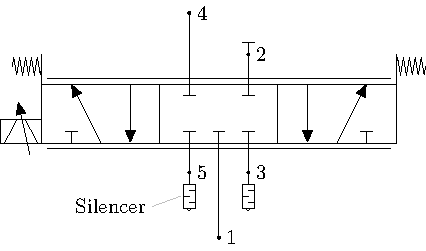
\includegraphics[scale=1]{5_3_proportional_valve.pdf}};
\draw[spy] (1)++(-.7,.1)rectangle++(1,.8)++(0,-.4)--(Pic); 

%%%%%%%%%%%%%%%%% SEPERATOR %%%%%%%%%%%%%%%

\draw[help] (-2.3,2.9)node[above right,scale=3, align=left]{\textsf{Discrete} \\ \textsf{Channel}}node[below right, scale=3]{\textsf{Continous Channel}}--++(20.5,0);

%%%%%%%%%%%%%%%%% DISCRETE %%%%%%%%%%%%%%%%
\begin{scope}[yshift=5cm]
% Vacuum Pump
\path (15,1)coordinate(0);
\draw (0)--++(0,-.25)++(0,-0.75)coordinate(C)circle(.75)++(0,-.75)--++(0,-.25);
\draw ($(C)+(270-50:.75)$)--($(C)+(90+15:.75)$);
\draw ($(C)+(270+50:.75)$)--($(C)+(90-15:.75)$);
\draw (0)++(0,-1)++(185:.75)--++(-.5,0)coordinate(X);
\draw (0)++(0,-1)++(175:.75)--++(-.5,0)--(X);
\path (0)++(.75,-1)node[right]{Vacuum Pump};
\fill (0)circle(.03)++(0,-2)coordinate(0);

% Discrete Valves
\foreach[count=\i] \x in {13,11.5,10,8.5}{
	\pvalve{\x}{0}
	\draw (0)--(1);
	\pgfmathtruncatemacro{\j}{5-\i}
	\draw[fill] (4)--++(0,.7)circle(.03)node[above]{D\j};
	\ifnum\i<4 
		\fill (1)circle(.03);
	\fi
	\path (1)coordinate(0);
}

% Nahaufnahme Discrete Valve
\path (2,-.5)node[right, spyfill](Pic2){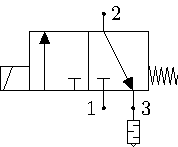
\includegraphics[scale=1]{3_2_discrete_valve.pdf}};
\draw[spy] (1)++(-.7,.1)rectangle++(1,.8)++(-1,-.4)--(Pic2); 
\end{scope}

\end{tikzpicture}
\end{document}